% =====================================================================
%  Python for Programmers -- a compact Beamer deck
%  Build:   latexmk -xelatex python-for-programmers.tex
%  Figures: python figures/make_figures.py   (numpy, pandas, matplotlib)
% =====================================================================
\documentclass[aspectratio=169,9pt]{beamer}

\usetheme[progressbar=frametitle, numbering=fraction,
          sectionpage=progressbar, block=fill]{metropolis}
\setbeamersize{text margin left=0.6cm, text margin right=0.6cm}

\usepackage{fontspec}
\setsansfont{FiraSans}[Extension=.otf, UprightFont=*-Book,
  BoldFont=*-SemiBold, ItalicFont=*-BookItalic, BoldItalicFont=*-SemiBoldItalic]
\setmonofont{FiraMono}[Extension=.otf, UprightFont=*-Regular,
  BoldFont=*-Medium, Scale=0.92]

\usepackage{listings}
\usepackage{booktabs}
\usepackage{tabularx}
\usepackage{graphicx}
\usepackage{tikz}
\usepackage{fontawesome5}
\graphicspath{{figures/}}

% ---------------------------------------------------------------- colors
\definecolor{ink}{HTML}{1F2430}
\definecolor{ink2}{HTML}{52514E}
\definecolor{pyblue}{HTML}{2A78D6}
\definecolor{pyorange}{HTML}{EB6834}
\definecolor{pyaqua}{HTML}{1BAF7A}
\definecolor{codebg}{HTML}{F4F5F7}
\definecolor{kw}{HTML}{1F5FB4}
\definecolor{str}{HTML}{0E7A52}
\definecolor{cmt}{HTML}{7A7D85}
\definecolor{bi}{HTML}{B4461A}

\setbeamercolor{normal text}{fg=ink, bg=white}
\setbeamercolor{frametitle}{fg=white, bg=ink}
\setbeamercolor{progress bar}{fg=pyblue, bg=pyblue!20}
\setbeamercolor{alerted text}{fg=pyorange!90!black}
\setbeamercolor{block title}{fg=ink, bg=pyblue!14}
\setbeamercolor{block body}{fg=ink, bg=pyblue!5}
\setbeamercolor{block title alerted}{fg=ink, bg=pyorange!18}
\setbeamercolor{block body alerted}{fg=ink, bg=pyorange!6}
\setbeamercolor{block title example}{fg=ink, bg=pyaqua!18}
\setbeamercolor{block body example}{fg=ink, bg=pyaqua!6}
\setbeamerfont{block title}{series=\bfseries}
\setbeamerfont{title}{size=\huge, series=\bfseries}
\setbeamerfont{subtitle}{size=\large}
\setbeamertemplate{itemize item}{\color{pyblue}\scriptsize$\blacktriangleright$}
\setbeamertemplate{itemize subitem}{\color{ink2}\scriptsize$\bullet$}

% --------------------------------------------------------------- listings
\newcommand{\codesize}{\fontsize{7.4}{8.9}\selectfont}
\lstdefinestyle{py}{
  language=Python,
  basicstyle=\ttfamily\codesize\color{ink},
  keywordstyle=\color{kw}\bfseries,
  stringstyle=\color{str},
  commentstyle=\color{cmt}\itshape,
  morekeywords={True,False,None,nonlocal,yield,with,as,lambda,match,case,async,await},
  deletekeywords={print},
  emph={print,len,range,enumerate,zip,sorted,sum,min,max,isinstance,type,
        int,float,str,list,dict,set,tuple,open,super,map,filter,any,all,
        abs,round,iter,next,repr,bool,divmod,frozenset,reversed,property,
        staticmethod,classmethod,dataclass},
  emphstyle=\color{bi},
  morestring=[s]{"""}{"""},
  showstringspaces=false, columns=fullflexible, keepspaces=true,
  upquote=true, tabsize=4,
  backgroundcolor=\color{codebg},
  frame=single, framerule=0pt, framesep=3pt,
  xleftmargin=3pt, xrightmargin=3pt,
  aboveskip=3pt, belowskip=3pt,
}
\lstdefinestyle{out}{
  style=py, language={}, basicstyle=\ttfamily\codesize\color{ink2},
  backgroundcolor=\color{white}, frame=leftline, framerule=1.2pt,
  rulecolor=\color{pyaqua}, keywordstyle={}, emph={}, commentstyle={},
}
\lstdefinestyle{sh}{
  style=py, language=bash, morekeywords={python,pip,source,uv},
  emph={}, morecomment=[l]{\#},
}
\lstset{style=py}
\lstdefinestyle{inl}{style=py, basicstyle=\ttfamily\color{ink},
  backgroundcolor={}, frame=none, keywordstyle=\color{ink}, emphstyle=\color{ink},
  stringstyle=\color{ink}, commentstyle=\color{ink}}
\lstMakeShortInline[style=inl]|

% helpers
\newcommand{\cc}[1]{\texttt{#1}}                      % code inside arguments
\newcommand{\hint}[1]{{\small\color{ink2}#1}}  % small grey remark
\newcommand{\gr}[1]{\textsf{\color{ink2}#1}}                % grey prose in tables
\newcommand{\head}[1]{{\color{pyblue!80!black}\bfseries #1}\par\vspace{1pt}}

% ------------------------------------------------------------------- meta
\title{Python for Programmers}
\subtitle{The language \textperiodcentered{} NumPy
          \textperiodcentered{} pandas \textperiodcentered{} Matplotlib}
\author{Youssef Alikhani}
\date{\today}

\begin{document}

\maketitle

% =====================================================================
\begin{frame}[fragile]{Agenda}
\begin{columns}[T]
\column{0.50\textwidth}
\begin{enumerate}\setlength\itemsep{6pt}
  \item \textbf{The language}\\
        \hint{mental model, syntax, types, collections, control flow,
        functions, classes, errors, files, generators, decorators, modules}
  \item \textbf{NumPy}\\
        \hint{ndarray, indexing, vectorization, broadcasting}
  \item \textbf{pandas}\\
        \hint{Series / DataFrame, selection, cleaning, group-by, joins}
  \item \textbf{Matplotlib}\\
        \hint{Figure / Axes model, plot types, an end-to-end example}
\end{enumerate}
\column{0.44\textwidth}
\begin{exampleblock}{Assumptions}
You already program (C/C++, Java, C\#, JS, \ldots). We skip
\emph{what a variable is} and focus on \alert{what is different in
Python} and how to write it \emph{idiomatically}.
\end{exampleblock}
\begin{block}{Conventions}
|# -> value| shows what a line evaluates to.
All outputs were produced by running the code
(Python 3.12, NumPy 2.5, pandas 3.1, Matplotlib 3.11).
\end{block}
\end{columns}
\end{frame}

% =====================================================================
\section{The Language}
% =====================================================================

\begin{frame}[fragile]{Python in one slide}
\begin{columns}[T]
\column{0.54\textwidth}
\begin{itemize}\setlength\itemsep{3pt}
  \item \textbf{Interpreted}: source $\rightarrow$ bytecode $\rightarrow$
        CPython VM. No build step; a REPL for exploring.
  \item \textbf{Dynamic \emph{and} strong typing}: names have no type,
        objects do. |"1" + 1| raises \alert{TypeError}.
  \item \textbf{Everything is an object}: ints, functions, classes,
        modules can all be passed around as values.
  \item \textbf{Indentation is syntax}: 4 spaces instead of braces,
        no semicolons.
  \item \textbf{Automatic memory}: reference counting + cycle GC.
  \item \textbf{Batteries included}: rich standard library plus a huge
        ecosystem on PyPI (|pip install ...|).
  \item \textbf{Trade-off}: pure-Python loops are slow, so heavy work
        is pushed into C libraries (NumPy, pandas, \ldots).
\end{itemize}
\column{0.42\textwidth}
\begin{lstlisting}
def fizzbuzz(n: int) -> str:
    if n % 15 == 0:
        return "FizzBuzz"
    if n % 3 == 0:
        return "Fizz"
    if n % 5 == 0:
        return "Buzz"
    return str(n)

for i in range(9, 16):
    print(fizzbuzz(i), end=" ")
\end{lstlisting}
\begin{lstlisting}[style=out]
Fizz Buzz 11 Fizz 13 14 FizzBuzz
\end{lstlisting}
\begin{lstlisting}[style=sh]
$ python fizz.py     # run a script
$ python             # interactive REPL
\end{lstlisting}
\end{columns}
\end{frame}

% ---------------------------------------------------------------------
\begin{frame}{Rosetta stone: C-family $\rightarrow$ Python}
\small
\renewcommand{\arraystretch}{1.12}
\begin{tabularx}{\textwidth}{@{}l>{\ttfamily}X>{\ttfamily}X@{}}
\toprule
\textbf{Concept} & \normalfont\textbf{C++ / Java / JS} & \normalfont\textbf{Python}\\
\midrule
Block            & if (x) \{ \ldots{} \}            & if x: \gr{(then an indented block)}\\
Declaration      & int n = 5;                       & n = 5 \\
Null / booleans  & null, true, false                & None, True, False \\
Logic            & \&\&\ \ \textbar\textbar\ \ !    & and\ \ or\ \ not \\
Ternary          & c ? a : b                        & a if c else b \\
Counting loop    & for (int i = 0; i < n; i++)      & for i in range(n): \\
For-each         & for (auto x : xs)                & for x in xs: \\
Increment        & i++                              & i += 1 \\
Dynamic array    & vector<T>, ArrayList<T>          & list\ \ \ [1, 2, 3] \\
Hash map         & unordered\_map, HashMap          & dict\ \ \ \{"k": 1\} \\
Receiver         & this \gr{(implicit)}             & self \gr{(explicit first parameter)} \\
Interfaces       & interface, abstract class        & duck typing, Protocol, ABC \\
Errors           & try \{\} catch (E e) \{\}        & try: \ldots{} except E as e: \\
Switch           & switch (x) \{ case 1: \ldots{} \} & match x: case 1: \ldots \\
\bottomrule
\end{tabularx}
\end{frame}

% ---------------------------------------------------------------------
\begin{frame}[fragile]{Tooling \& project setup}
\begin{columns}[T]
\column{0.54\textwidth}
\head{One virtual environment per project}
\begin{lstlisting}[style=sh]
python -m venv .venv             # create
.venv\Scripts\activate           # Windows
source .venv/bin/activate        # macOS / Linux
pip install numpy pandas matplotlib
pip freeze > requirements.txt    # pin versions
pip install -r requirements.txt  # reproduce
\end{lstlisting}
\hint{\textbf{uv} is a fast modern alternative:
\cc{uv init}, \cc{uv add pandas}, \cc{uv run main.py}.}

\medskip
\head{Editors}
\begin{itemize}
  \item VS Code (+ Python extension), PyCharm
  \item Jupyter notebooks: the standard for exploratory data work
\end{itemize}
\column{0.42\textwidth}
\begin{block}{Style: PEP 8 in five rules}
\begin{itemize}
  \item 4 spaces per indent, no tabs
  \item |snake_case|: variables, functions, modules
  \item |PascalCase|: classes
  \item |UPPER_CASE|: constants (by convention)
  \item |_leading_underscore|: internal
\end{itemize}
\end{block}
\begin{exampleblock}{Quality tools}
\textbf{ruff} lint + format \textperiodcentered{}
\textbf{mypy}/\textbf{pyright} type checks \textperiodcentered{}
\textbf{pytest} tests \textperiodcentered{}
\textbf{ipython} better REPL
\end{exampleblock}
\end{columns}
\end{frame}

% ---------------------------------------------------------------------
\begin{frame}[fragile]{Syntax basics}
\begin{columns}[T]
\column{0.55\textwidth}
\begin{lstlisting}
# Comments start with a hash
import math

MAX_RETRIES = 3          # "constant" by convention
user_name = "ada"        # no declarations, no types
x = y = 0                # chained assignment
a, b = 1, 2              # tuple unpacking
a, b = b, a              # swap, no temp variable

def area(r):             # colon + indented block
    """Docstring: shown by help(area)."""
    if r < 0:
        raise ValueError("negative radius")
    return math.pi * r ** 2

total = (1 + 2 +         # implicit line continuation
         3 + 4)          # inside (), [], {}
print(f"{area(2):.2f}")  # -> 12.57
\end{lstlisting}
\column{0.41\textwidth}
\begin{itemize}\setlength\itemsep{5pt}
  \item A variable is a \textbf{name bound to an object}.
        Assignment never copies; it attaches a label.
  \item Inspect types with |type(x)|; test them with
        |isinstance(x, int)|.
  \item Case-sensitive. Keywords (|if|, |def|, |class|, |lambda|,
        \ldots) are reserved.
  \item |pass| is the empty statement.
  \item |input()| reads a line as |str|;
        |print(a, b, sep=", ")| writes.
\end{itemize}
\end{columns}
\end{frame}

% ---------------------------------------------------------------------
\begin{frame}[fragile]{Numbers, booleans \& operators}
\begin{columns}[T]
\column{0.55\textwidth}
\begin{lstlisting}
2 ** 100        # -> 1267650600228229401496703205376
                #    ints never overflow
7 / 2           # -> 3.5   true division: always float
7 // 2          # -> 3     floor division
-7 // 2         # -> -4    floors toward -infinity
-7 % 3          # -> 2     sign follows the divisor
divmod(17, 5)   # -> (3, 2)
3 + 4j          # complex numbers are built in

0.1 + 0.2 == 0.3              # -> False (IEEE 754)
math.isclose(0.1 + 0.2, 0.3)  # -> True

1 < x <= 10            # chained comparison
x is None              # identity: use it for None
"" or "default"        # -> 'default'
if (n := len(data)) > 3:   # walrus: assign + test
    print(n)
\end{lstlisting}
\column{0.41\textwidth}
\begin{block}{Truthiness}
\emph{Falsy}: |False|, |None|, |0|, |0.0|, |""|, |[]|, |{}|,
|set()|. Everything else is truthy, so write |if items:|,
not |if len(items) > 0:|.
\end{block}
\begin{itemize}\setlength\itemsep{3pt}
  \item |and| / |or| short-circuit and return an \emph{operand}.
  \item |==| compares values, |is| compares identity.
  \item Bitwise: \cc{\&\ \ \textbar\ \ \^{}\ \ \textasciitilde\ \ <{}<\ \ >{}>};
        membership: |in|, |not in|.
  \item No |++| / |--|; use |+=| / |-=|.
\end{itemize}
\end{columns}
\end{frame}

% ---------------------------------------------------------------------
\begin{frame}[fragile]{Strings}
\begin{columns}[T]
\column{0.54\textwidth}
\begin{lstlisting}
s = "Hello, Python"     # ' and " are equivalent
s[0], s[-1]             # -> ('H', 'n')
s[7:]                   # -> 'Python'
s[::-1]                 # -> 'nohtyP ,olleH'
s.upper()               # -> 'HELLO, PYTHON'
s.split(", ")           # -> ['Hello', 'Python']
"-".join(["a", "b"])    # -> 'a-b'
"  hi ".strip()         # -> 'hi'
"abc".replace("b", "B") # -> 'aBc'
"py" in "python"        # -> True
s.startswith("He"), s.find("P"), len(s)
s[0] = "J"              # TypeError: immutable
\end{lstlisting}
\hint{Slicing \cc{[start:stop:step]} works on every sequence;
\cc{stop} is exclusive, negative indices count from the end.}
\column{0.42\textwidth}
\head{f-strings: the way to format}
\begin{lstlisting}
name, pi = "Ada", 3.14159
f"{pi:.2f} | {1234567:,} | {0.25:.0%}"
# -> '3.14 | 1,234,567 | 25%'
f"{name!r:>6}|"     # -> " 'Ada'|"
f"{pi=}"            # -> 'pi=3.14159'
\end{lstlisting}
\head{Other literals}
\begin{lstlisting}
r"C:\new\table"     # raw: no escapes
"""Triple quotes span
multiple lines"""
b"\x00\xff"         # bytes, not str
"caf\u00e9".encode("utf-8")
\end{lstlisting}
\hint{\cc{str} is Unicode text, \cc{bytes} is binary data;
convert with \cc{.encode()} / \cc{.decode()}.}
\end{columns}
\end{frame}

% ---------------------------------------------------------------------
\begin{frame}[fragile]{Built-in collections}
\small
\renewcommand{\arraystretch}{1.2}
\begin{tabularx}{\textwidth}{@{}l>{\ttfamily}lcc>{\raggedright\arraybackslash}X@{}}
\toprule
\textbf{Type} & \normalfont\textbf{Literal} & \textbf{Mutable} & \textbf{Ordered} & \textbf{Use it for}\\
\midrule
\cc{list}      & [1, "a", 2.0]    & \checkmark & \checkmark & dynamic array; \cc{append} $O(1)$, \cc{in} $O(n)$ \\
\cc{tuple}     & (1, 2)\ \ \textsf{or}\ \ 1, 2 & -- & \checkmark & fixed records, multiple return values; hashable, so usable as a dict key \\
\cc{dict}      & \{"id": 7, "ok": True\} & \checkmark & insertion & hash map, $O(1)$ average lookup; keys must be hashable \\
\cc{set}       & \{1, 2, 3\}      & \checkmark & -- & unique items, $O(1)$ \cc{in}, set algebra \\
\cc{frozenset} & frozenset(\{1\}) & -- & -- & immutable, hashable set \\
\bottomrule
\end{tabularx}

\vspace{8pt}
\normalsize
\begin{columns}[T]
\column{0.48\textwidth}
\begin{alertblock}{Classic traps}
|{}| is an empty \textbf{dict}; use |set()| for an empty set.\\
|(1)| is just |1|; a one-element tuple is |(1,)|.
\end{alertblock}
\column{0.48\textwidth}
\begin{block}{All of them are iterable}
|len()|, |in|, |for x in c|, |sorted(c)|, |min| / |max| / |sum|
and unpacking work on every collection.
\end{block}
\end{columns}
\end{frame}

% ---------------------------------------------------------------------
\begin{frame}[fragile]{Collections in practice}
\begin{columns}[T]
\column{0.49\textwidth}
\head{list \& tuple}
\begin{lstlisting}
xs = [3, 1, 4]
xs.append(1); xs.extend([5, 9])
xs.insert(0, 2); xs.pop(); xs.remove(4)
xs.sort()                # in place, returns None
sorted(xs, reverse=True) # new list
xs[1:3] = [7, 7]         # slice assignment

first, *rest = [1, 2, 3, 4]  # 1, [2, 3, 4]
[*xs, 0]                 # unpack into a literal
x, y = (3, 4)            # tuple unpacking
\end{lstlisting}
\head{set}
\begin{lstlisting}
a, b = {1, 2}, {2, 3}
a | b, a & b, a - b      # {1, 2, 3} {2} {1}
\end{lstlisting}
\column{0.49\textwidth}
\head{dict}
\begin{lstlisting}
d = {"a": 1}
d["b"] = 2               # insert / update
d["z"]                   # KeyError
d.get("z", 0)            # -> 0 (default)
d.setdefault("c", []).append(1)
for k, v in d.items():   # .keys(), .values()
    print(k, v)
d | {"e": 5}             # merge -> new dict
{**d, "e": 5}            # same, via unpacking
del d["a"]
\end{lstlisting}
\head{collections module}
\begin{lstlisting}
from collections import Counter, defaultdict
Counter("mississippi").most_common(2)
# -> [('i', 4), ('s', 4)]
groups = defaultdict(list) # missing key -> []
groups["k"].append(1)
\end{lstlisting}
\end{columns}
\end{frame}

% ---------------------------------------------------------------------
\begin{frame}[fragile]{References \& mutability: the \#1 source of surprises}
\begin{columns}[T]
\column{0.53\textwidth}
\begin{lstlisting}
a = [1, 2, 3]
b = a              # same object, NOT a copy
b.append(4)
print(a)           # -> [1, 2, 3, 4]
c = a.copy()       # shallow; copy.deepcopy() = deep

grid = [[0] * 3] * 3   # 3 references to ONE row
grid[0][0] = 1
# -> [[1, 0, 0], [1, 0, 0], [1, 0, 0]]
grid = [[0] * 3 for _ in range(3)]   # correct

def add(x, lst=[]):    # default evaluated ONCE
    lst.append(x)
    return lst
add(1); add(2)         # -> [1, 2]  shared!
def add(x, lst=None):  # the idiom
    lst = [] if lst is None else lst
    ...
\end{lstlisting}
\column{0.43\textwidth}
\begin{block}{Mutable vs immutable}
\textbf{Mutable}: |list|, |dict|, |set|, most user objects.\\
\textbf{Immutable}: |int|, |float|, |str|, |tuple|, |bytes|,
|frozenset|.
\end{block}
\begin{block}{Arguments: ``call by sharing''}
A function receives a reference to the caller's object:
\emph{mutating} it (|lst.append|) is visible to the caller,
\emph{rebinding} it (|lst = []|) is not.
\end{block}
\begin{alertblock}{Rule of thumb}
Never use a mutable object as a default argument.
\end{alertblock}
\end{columns}
\end{frame}

% ---------------------------------------------------------------------
\begin{frame}[fragile]{Control flow: \texttt{if} and \texttt{match}}
\begin{columns}[T]
\column{0.42\textwidth}
\begin{lstlisting}
if score >= 90:
    grade = "A"
elif score >= 75:
    grade = "B"
else:
    grade = "C"

# conditional expression (ternary)
status = "adult" if age >= 18 else "minor"

if debug:
    pass        # empty block placeholder
\end{lstlisting}
\hint{No parentheses needed around conditions. Combine them with
\cc{and} / \cc{or} / \cc{not}.}
\column{0.54\textwidth}
\head{Structural pattern matching (3.10+)}
\hint{A switch that \emph{destructures}. No fall-through, no
\cc{break}.}
\begin{lstlisting}
match command.split():
    case ["go", direction]:         # binds direction
        move(direction)
    case ["quit" | "exit"]:         # alternatives
        stop()
    case ["say", *words] if words:  # guard
        print(" ".join(words))
    case _:                         # default
        print("unknown command")

match event:
    case {"type": "click", "pos": (x, y)}:
        handle_click(x, y)          # dict + tuple
    case Point(x=0, y=0):           # class pattern
        print("origin")
\end{lstlisting}
\end{columns}
\end{frame}

% ---------------------------------------------------------------------
\begin{frame}[fragile]{Loops}
\begin{columns}[T]
\column{0.55\textwidth}
\begin{lstlisting}
for x in [10, 20, 30]:          # iterate items
    print(x)
for i in range(5): ...          # 0..4
for i in range(10, 0, -3): ...  # 10, 7, 4, 1
for i, name in enumerate(names, start=1): ...
for name, age in zip(names, ages): ...

while queue:
    item = queue.pop()
    if item == "STOP":
        break

for n in numbers:
    if n % 2 == 0:
        print("found", n)
        break
else:            # runs only if the loop did not break
    print("no even number")
\end{lstlisting}
\column{0.41\textwidth}
\begin{itemize}\setlength\itemsep{5pt}
  \item No C-style |for(;;)|, no |do-while|: you iterate
        \emph{over things}.
  \item Need the index? |enumerate|, not |range(len(xs))|.
  \item Parallel sequences? |zip| (stops at the shortest).
  \item |range| is lazy: |range(10**9)| costs no memory.
  \item Don't add/remove items of a list while looping over it;
        build a new list instead.
\end{itemize}
\end{columns}
\end{frame}

% ---------------------------------------------------------------------
\begin{frame}[fragile]{Comprehensions}
\begin{columns}[T]
\column{0.57\textwidth}
\begin{lstlisting}
nums = [3, 1, 4, 1, 5, 9, 2, 6]

[n * n for n in nums if n % 2 == 0]  # -> [16, 4, 36]
{n % 3 for n in nums}                # -> {0, 1, 2}
{w: len(w) for w in ["hi", "hey"]}
# -> {'hi': 2, 'hey': 3}

sum(n * n for n in nums)   # -> 173
                           # generator expression:
                           # lazy, no list is built
any(n > 8 for n in nums)   # -> True

["even" if n % 2 == 0 else "odd" for n in nums]

[(x, y) for x in range(2) for y in "ab"]
# -> [(0, 'a'), (0, 'b'), (1, 'a'), (1, 'b')]
\end{lstlisting}
\column{0.39\textwidth}
\begin{block}{Shape}
\centering
\cc{[\alert{expr} for x in it if \alert{cond}]}\\[3pt]
\hint{\cc{[]} list \textperiodcentered{} \cc{\{\}} set
\textperiodcentered{} \cc{\{k: v\}} dict \textperiodcentered{}
\cc{()} generator}
\end{block}
\begin{itemize}\setlength\itemsep{5pt}
  \item Replaces most |map| / |filter| and
        ``create a list, then append'' loops.
  \item Usually faster than the equivalent loop.
  \item Keep them short. If it needs more than a line or two,
        write a normal loop.
\end{itemize}
\end{columns}
\end{frame}

% ---------------------------------------------------------------------
\begin{frame}[fragile]{Functions}
\begin{columns}[T]
\column{0.58\textwidth}
\begin{lstlisting}
def greet(name: str, greeting: str = "Hello") -> str:
    """Return a greeting."""
    return f"{greeting}, {name}!"

greet("Ada")                      # positional
greet(greeting="Hi", name="Ada")  # keyword, any order

def f(a, b, /, c, *, d=1, **kw):
    return a, b, c, d, kw
f(1, 2, 3, d=4, e=5)    # -> (1, 2, 3, 4, {'e': 5})

def log(*args, **kwargs):          # variadic
    print(args, kwargs)
log(1, 2, level="info") # -> (1, 2) {'level': 'info'}
log(*[1, 2], **{"level": "info"})  # unpack at call

def min_max(xs):
    return min(xs), max(xs)        # returns a tuple
lo, hi = min_max([3, 1, 4])
\end{lstlisting}
\column{0.38\textwidth}
\begin{block}{Parameter kinds}
\cc{a, b, /}\ \ positional-only\\
\cc{c}\ \ positional or keyword\\
\cc{*, d=1}\ \ keyword-only\\
\cc{*args}\ \ extra positionals (tuple)\\
\cc{**kw}\ \ extra keywords (dict)
\end{block}
\begin{itemize}\setlength\itemsep{3pt}
  \item \textbf{Type hints are not enforced} at runtime; IDEs and
        mypy/pyright use them.
  \item No overloading by signature: use defaults and keywords.
  \item No |return| means |None| is returned.
\end{itemize}
\end{columns}
\end{frame}

% ---------------------------------------------------------------------
\begin{frame}[fragile]{Functions are objects: lambdas, closures, scope}
\begin{columns}[T]
\column{0.55\textwidth}
\begin{lstlisting}
square = lambda x: x * x     # one-expression function
people = [("bob", 25), ("ann", 31), ("cy", 19)]
sorted(people, key=lambda p: p[1])
# -> [('cy', 19), ('bob', 25), ('ann', 31)]

def make_counter():
    count = 0
    def inc():
        nonlocal count       # rebind enclosing name
        count += 1
        return count
    return inc               # closure keeps count

c = make_counter()
c(); c()                     # -> 2

list(map(str.upper, ["a", "b"]))   # -> ['A', 'B']
from functools import reduce
reduce(lambda a, b: a * b, [1, 2, 3, 4])   # -> 24
\end{lstlisting}
\column{0.41\textwidth}
\begin{block}{Scope rule: LEGB}
Lookup order: \textbf{L}ocal $\rightarrow$ \textbf{E}nclosing
$\rightarrow$ \textbf{G}lobal $\rightarrow$ \textbf{B}uilt-in.
|global x| / |nonlocal x| are needed only to \emph{rebind}.
\end{block}
\begin{alertblock}{Gotchas}
\begin{itemize}
  \item |if| / |for| do \textbf{not} create a scope: the loop
        variable survives the loop.
  \item Late binding: |[lambda: i for i in range(3)]| all
        return \cc{2}. Fix with |lambda i=i: i|.
\end{itemize}
\end{alertblock}
\end{columns}
\end{frame}

% ---------------------------------------------------------------------
\begin{frame}[fragile]{Classes}
\begin{columns}[T]
\column{0.60\textwidth}
\begin{lstlisting}
class Account:
    bank = "PyBank"              # class attribute
    def __init__(self, owner: str, balance: float = 0):
        self.owner = owner       # instance attributes
        self._balance = balance  # _ = internal
    @property
    def balance(self) -> float:  # read as acc.balance
        return self._balance
    def deposit(self, amount: float) -> None:
        if amount <= 0:
            raise ValueError("amount must be positive")
        self._balance += amount
    def __repr__(self) -> str:   # used by the REPL
        return f"Account({self.owner!r}, {self._balance})"

acc = Account("Ada", 100)        # no `new`
acc.deposit(50)
acc.balance                      # -> 150
acc                              # -> Account('Ada', 150)
\end{lstlisting}
\column{0.36\textwidth}
\begin{itemize}\setlength\itemsep{5pt}
  \item |self| is an explicit |this|: the first parameter of every
        method.
  \item |__init__| initializes; |self.x = ...| creates attributes.
  \item \textbf{No access modifiers}: |_x| means ``internal'' by
        convention; |__x| is name-mangled.
  \item Prefer plain attributes; switch to |@property| later
        without breaking callers. No |getX()| / |setX()|.
  \item |@classmethod|: alternative constructors.
\end{itemize}
\end{columns}
\end{frame}

% ---------------------------------------------------------------------
\begin{frame}[fragile]{Inheritance, dunder methods \& dataclasses}
\begin{columns}[T]
\column{0.53\textwidth}
\begin{lstlisting}
class Savings(Account):                 # inherits
    def __init__(self, owner, balance=0, rate=0.02):
        super().__init__(owner, balance)
        self.rate = rate
    def add_interest(self):
        self.deposit(self.balance * self.rate)
\end{lstlisting}
\head{dataclass: boilerplate generated for you}
\begin{lstlisting}
from dataclasses import dataclass
# generates __init__, __repr__, __eq__
@dataclass(frozen=True)
class Point:
    x: float
    y: float = 0.0
    def __add__(self, other):   # overloads +
        return Point(self.x + other.x,
                     self.y + other.y)
Point(1, 2) + Point(3)    # -> Point(x=4, y=2.0)
\end{lstlisting}
\column{0.43\textwidth}
\head{Dunder (``double underscore'') methods}
\footnotesize
\begin{tabular}{@{}>{\ttfamily}l>{\ttfamily}l@{}}
\toprule
\normalfont\textbf{Define} & \normalfont\textbf{To support}\\
\midrule
\_\_repr\_\_, \_\_str\_\_       & repr(o), print(o) \\
\_\_eq\_\_, \_\_lt\_\_          & ==, <, sorted() \\
\_\_len\_\_, \_\_getitem\_\_    & len(o), o[i] \\
\_\_iter\_\_, \_\_contains\_\_  & for, in \\
\_\_add\_\_, \_\_mul\_\_        & +, * \\
\_\_call\_\_                    & o() \\
\_\_enter\_\_, \_\_exit\_\_     & with o: \\
\bottomrule
\end{tabular}

\normalsize
\vspace{6pt}
\begin{block}{Duck typing}
Anything with |.read()| can stand in for a file. Static checks:
|typing.Protocol|.
\end{block}
\end{columns}
\end{frame}

% ---------------------------------------------------------------------
\begin{frame}[fragile]{Exceptions}
\begin{columns}[T]
\column{0.58\textwidth}
\begin{lstlisting}
class InvalidAge(ValueError): pass   # custom error
def parse_age(text: str) -> int:
    try:
        age = int(text)
    except ValueError as e:
        raise InvalidAge(f"bad age: {text!r}") from e
    if age < 0:
        raise InvalidAge("age must be >= 0")
    return age
try:
    age = parse_age("abc")
except InvalidAge as e:
    print("error:", e)  # -> error: bad age: 'abc'
except (TypeError, KeyError):   # several at once
    ...
else:
    print("ok", age)    # only if nothing was raised
finally:
    print("cleanup")    # always runs
\end{lstlisting}
\column{0.38\textwidth}
\begin{block}{EAFP over LBYL}
``Easier to Ask Forgiveness than Permission'':
\begin{lstlisting}
try:
    value = cache[key]
except KeyError:
    value = cache[key] = compute(key)
\end{lstlisting}
\end{block}
\begin{itemize}\setlength\itemsep{3pt}
  \item Common: |ValueError|, |TypeError|, |KeyError|,
        |IndexError|, |AttributeError|, |FileNotFoundError|.
  \item Never a bare |except:|; catch the narrowest type.
\end{itemize}
\end{columns}
\end{frame}

% ---------------------------------------------------------------------
\begin{frame}[fragile]{Files \& context managers}
\begin{columns}[T]
\column{0.57\textwidth}
\begin{lstlisting}
from pathlib import Path
path = Path("data") / "notes.txt"  # OS-independent
path.parent.mkdir(exist_ok=True)

with open(path, "w", encoding="utf-8") as f:
    f.write("first line\n")   # closed automatically,
                              # even on an error
with open(path, encoding="utf-8") as f:   # mode "r"
    for line in f:            # lazy, line by line
        print(line.rstrip())

text = path.read_text(encoding="utf-8")   # all at once
path.suffix, path.stem        # -> ('.txt', 'notes')
list(Path(".").glob("*.csv")) # find files

import json
cfg = json.loads(Path("config.json").read_text())
Path("out.json").write_text(json.dumps(cfg, indent=2))
\end{lstlisting}
\column{0.39\textwidth}
\head{File modes}
\footnotesize
\begin{tabular}{@{}>{\ttfamily}ll@{}}
\toprule
r & read (default) \\
w & write, truncates first \\
a & append \\
x & create, fail if it exists \\
b & binary, e.g.\ \cc{"rb"} \\
\bottomrule
\end{tabular}

\normalsize
\vspace{6pt}
\begin{block}{\texttt{with} is general}
Works with any object that has |__enter__| / |__exit__|: locks,
DB connections, temp dirs. Write your own with
|@contextlib.contextmanager|.
\end{block}
\end{columns}
\end{frame}

% ---------------------------------------------------------------------
\begin{frame}[fragile]{Iterators \& generators}
\begin{columns}[T]
\column{0.55\textwidth}
\begin{lstlisting}
def fib():                 # a generator function
    a, b = 0, 1
    while True:
        yield a            # pause; resume on next()
        a, b = b, a + b

from itertools import islice
list(islice(fib(), 8))
# -> [0, 1, 1, 2, 3, 5, 8, 13]
g = fib()
next(g), next(g), next(g)  # -> (0, 1, 1)

def read_rows(path):       # streaming: O(1) memory
    with open(path) as f:
        for line in f:
            yield line.rstrip().split(",")

ir = (r for r in read_rows(p) if r[0] == "IR")
for row in ir: ...         # one row at a time
\end{lstlisting}
\column{0.41\textwidth}
\begin{block}{The iteration protocol}
|for x in obj| calls |iter(obj)|, then |next()| until
|StopIteration| is raised. Implement |__iter__| / |__next__|, or
just write a generator.
\end{block}
\begin{itemize}\setlength\itemsep{4pt}
  \item Generators are \textbf{lazy}: values are produced on
        demand. Ideal for infinite sequences, huge files, pipelines.
  \item A generator can be consumed \textbf{only once}.
  \item |itertools|: |chain|, |islice|, |groupby|, |product|,
        |combinations|, |accumulate|, \ldots
\end{itemize}
\end{columns}
\end{frame}

% ---------------------------------------------------------------------
\begin{frame}[fragile]{Decorators}
\begin{columns}[T]
\column{0.57\textwidth}
\begin{lstlisting}
import functools, time
def timed(func):                   # takes a function,
    @functools.wraps(func)
    def wrapper(*args, **kwargs):  # returns a new one
        t0 = time.perf_counter()
        result = func(*args, **kwargs)
        dt = time.perf_counter() - t0
        print(f"{func.__name__} took {dt:.3f}s")
        return result
    return wrapper

@timed            # same as: slow_sum = timed(slow_sum)
def slow_sum(n):
    return sum(range(n))

@functools.cache  # memoization for free
def fib(n):
    return n if n < 2 else fib(n - 1) + fib(n - 2)
fib(100)         # -> 354224848179261915075, instantly
\end{lstlisting}
\column{0.39\textwidth}
\begin{block}{Idea}
A decorator wraps a function (or class) to add behaviour: logging,
timing, caching, access checks, retries, registration.
\end{block}
\head{You will meet these often}
\begin{itemize}\setlength\itemsep{2pt}
  \item |@property|, |@classmethod|, |@staticmethod|
  \item |@dataclass|, |@functools.cache|
  \item |@contextlib.contextmanager|
  \item Frameworks: |@app.get("/")|, |@pytest.fixture|
\end{itemize}
\end{columns}
\end{frame}

% ---------------------------------------------------------------------
\begin{frame}[fragile]{Modules, packages \& the standard library}
\begin{columns}[T]
\column{0.50\textwidth}
\begin{lstlisting}
import math                 # use as math.sqrt(2)
import numpy as np          # alias (convention)
from pathlib import Path    # import one name
from shop.cart import Cart  # package = folder
# from x import *           # avoid
\end{lstlisting}
\begin{lstlisting}
# shop/cli.py
def main() -> None:
    ...

if __name__ == "__main__":  # True only when run
    main()                  # directly, not imported
\end{lstlisting}
\hint{Every \cc{.py} file is a module. Its top level runs once, on the
first import; later imports reuse the cached module.}
\column{0.46\textwidth}
\head{Batteries included}
\footnotesize
\renewcommand{\arraystretch}{1.08}
\begin{tabular}{@{}>{\ttfamily}l l@{}}
\toprule
collections        & Counter, defaultdict, deque \\
itertools, functools & iteration \& functional tools \\
pathlib, os, shutil & files and the OS \\
json, csv, sqlite3 & data formats, embedded DB \\
datetime           & dates, times, time zones \\
re                 & regular expressions \\
logging, argparse  & logs, command-line interfaces \\
subprocess         & run other programs \\
concurrent.futures & thread / process pools \\
asyncio            & async I/O \\
unittest           & tests (or 3rd-party pytest) \\
\bottomrule
\end{tabular}
\end{columns}
\end{frame}

% ---------------------------------------------------------------------
\begin{frame}{Pythonic idioms}
\small
\renewcommand{\arraystretch}{1.3}
\begin{tabular}{@{}>{\ttfamily\color{ink2}}l@{\hspace{2.2em}}>{\ttfamily}l@{}}
\toprule
\normalfont\textbf{Instead of \ldots} & \normalfont\textbf{write}\\
\midrule
for i in range(len(xs)): print(xs[i])      & for x in xs: \gr{or} for i, x in enumerate(xs): \\
if len(xs) == 0:                           & if not xs: \\
if x == None:                              & if x is None: \\
if type(x) == int:                         & if isinstance(x, int): \\
s = ""; for p in parts: s += p             & s = "".join(parts) \\
tmp = a; a = b; b = tmp                    & a, b = b, a \\
f = open(p); data = f.read(); f.close()    & with open(p) as f: data = f.read() \\
v = d[k] if k in d else 0                  & v = d.get(k, 0) \\
out = []; for x in xs: out.append(f(x))    & out = [f(x) for x in xs] \\
"\%s is \%d" \% (name, age)                & f"\{name\} is \{age\}" \\
if x > 0 and x < 10:                       & if 0 < x < 10: \\
\bottomrule
\end{tabular}

\vspace{8pt}
\hint{\faLightbulb[regular]\enspace Run \texttt{import this} for the
``Zen of Python'': \emph{Readability counts. Explicit is better than
implicit. There should be one obvious way to do it.}}
\end{frame}

% =====================================================================
\section{NumPy}
% =====================================================================

\begin{frame}[fragile]{Why NumPy? The \texttt{ndarray}}
\begin{columns}[T]
\column{0.42\textwidth}
\begin{itemize}\setlength\itemsep{4pt}
  \item An \textbf{N-dimensional array} of a single \textbf{dtype}
        (|int64|, |float64|, |bool|, \ldots) in contiguous memory.
  \item Operations run as compiled C loops, with no per-element
        Python overhead.
  \item The foundation of pandas, Matplotlib, SciPy, scikit-learn.
\end{itemize}
\begin{exampleblock}{Measured: sum of squares of $10^6$ floats}
\footnotesize
\begin{tabular}{@{}lr@{}}
pure Python \ \cc{sum(v*v for v in xs)} & 87\,ms \\
NumPy \ \cc{(x*x).sum()}               & 3\,ms \\
\end{tabular}\\[2pt]
\hint{About 30$\times$ faster on the machine that built these slides.}
\end{exampleblock}
\column{0.54\textwidth}
\begin{lstlisting}
import numpy as np

np.array([1, 2, 3])          # from a list; int64
np.zeros((2, 3)); np.ones(4); np.full((2, 2), 7)
np.arange(0, 10, 2)          # -> [0 2 4 6 8]
np.linspace(0, 1, 5)   # -> [0. 0.25 0.5 0.75 1.]
np.eye(3)                    # identity matrix
rng = np.random.default_rng(42)
rng.normal(0, 1, size=(3, 3))

a = np.arange(12).reshape(3, 4)  # -1 infers a dim
a.shape, a.ndim, a.size      # -> (3, 4) 2 12
a.dtype                      # -> int64
a.T.shape                    # -> (4, 3)
a.astype(np.float32)         # convert (copy)
a.tolist()                   # back to Python lists
\end{lstlisting}
\end{columns}
\end{frame}

% ---------------------------------------------------------------------
\begin{frame}[fragile]{Indexing, slicing \& boolean masks}
\begin{columns}[T]
\column{0.55\textwidth}
\begin{lstlisting}
a = np.arange(12).reshape(3, 4)
# [[ 0  1  2  3]
#  [ 4  5  6  7]
#  [ 8  9 10 11]]

a[1, 2]               # -> 6   (rather than a[1][2])
a[1]                  # -> [4 5 6 7]    row
a[:, 2]               # -> [ 2  6 10]   column
a[1:, ::2]            # -> [[ 4  6]
                      #     [ 8 10]]
a[a % 2 == 0]         # -> [ 0  2  4  6  8 10]
a[(a > 2) & (a < 6)]  # combine masks: & | ~
a[[0, 2]]             # rows 0 and 2 (fancy)
np.where(a > 5, a, 0) # element-wise if/else
a[a > 5] = 0          # masked assignment
\end{lstlisting}
\column{0.41\textwidth}
\begin{alertblock}{Slices are views, not copies}
\begin{lstlisting}[aboveskip=7pt]
row = a[0]
row[0] = 99
a[0, 0]          # -> 99  (a changed!)
safe = a[0].copy()
\end{lstlisting}
Basic slices share memory with the original: cheap, but writes go
through. Masks and fancy indexing return \textbf{copies}.
\end{alertblock}
\begin{block}{Axis convention}
Index order is |[row, column]|, i.e.\ |[axis 0, axis 1]|.
\end{block}
\end{columns}
\end{frame}

% ---------------------------------------------------------------------
\begin{frame}[fragile]{Vectorization \& broadcasting}
\begin{columns}[T]
\column{0.53\textwidth}
\begin{lstlisting}
x = np.array([1, 2, 3])
x * np.array([10, 20, 30])  # -> [10 40 90]
x * 2 + 1                   # -> [3 5 7]
np.sqrt(x); np.exp(x)       # ufuncs: element-wise

a = np.arange(12).reshape(3, 4)
a.sum()                # -> 66
a.sum(axis=0)          # -> [12 15 18 21]  per column
a.mean(axis=1)         # -> [1.5 5.5 9.5]  per row
a.max(), a.argmax(), a.std()

col = np.array([[10], [20], [30]])   # shape (3, 1)
a + col                # (3, 4) + (3, 1) -> (3, 4)
# [[10 11 12 13]
#  [24 25 26 27]
#  [38 39 40 41]]
\end{lstlisting}
\column{0.43\textwidth}
\begin{center}
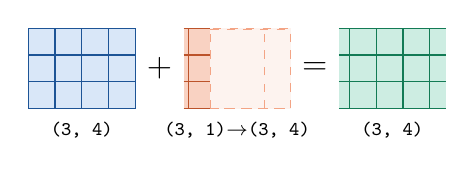
\begin{tikzpicture}[x=0.34cm, y=0.34cm, font=\scriptsize]
  \fill[pyblue!18] (0,0) rectangle (4,3);
  \draw[pyblue!70!black, step=1] (0,0) grid (4,3);
  \node at (2,-0.8) {\cc{(3, 4)}};
  \node at (4.9,1.5) {\large +};
  \fill[pyorange!30] (5.8,0) rectangle (6.8,3);
  \fill[pyorange!8] (6.8,0) rectangle (9.8,3);
  \draw[pyorange!80!black, step=1] (5.8,0) grid (6.8,3);
  \draw[pyorange!60, dashed] (6.8,0) grid (9.8,3);
  \draw[pyorange!60, dashed] (6.8,0) rectangle (9.8,3);
  \node at (7.8,-0.8) {\cc{(3, 1)}$\rightarrow$\cc{(3, 4)}};
  \node at (10.7,1.5) {\large =};
  \fill[pyaqua!22] (11.6,0) rectangle (15.6,3);
  \draw[pyaqua!70!black, step=1] (11.6,0) grid (15.6,3);
  \node at (13.6,-0.8) {\cc{(3, 4)}};
\end{tikzpicture}
\end{center}
\begin{block}{Broadcasting rules}
Compare shapes \textbf{right to left}. Two dimensions fit if they are
\textbf{equal} or one is \textbf{1} (it is stretched without copying).
Missing dimensions count as 1.
\end{block}
\begin{exampleblock}{Mindset}
Write \emph{array expressions}, not loops. A Python |for| over an
array is usually a missed vectorization.
\end{exampleblock}
\end{columns}
\end{frame}

% ---------------------------------------------------------------------
\begin{frame}[fragile]{Linear algebra, random numbers \& the toolbox}
\begin{columns}[T]
\column{0.52\textwidth}
\begin{lstlisting}
A = np.array([[2, 1], [1, 3]])
b = np.array([3, 5])
A @ A                    # matrix product
# -> [[ 5  5]
#     [ 5 10]]
np.linalg.solve(A, b)    # -> [0.8 1.4]  (Ax = b)
np.linalg.inv(A); np.linalg.det(A)
np.linalg.eig(A); np.linalg.norm(b)

rng = np.random.default_rng(seed=42)  # reproducible
rng.integers(0, 10, size=5)   # -> [0 7 6 4 4]
rng.normal(loc=0, scale=1, size=1000)
rng.choice(["a", "b"], size=3)
rng.permutation(10)
\end{lstlisting}
\hint{\cc{*} is element-wise; \cc{@} is matrix multiplication.}
\column{0.44\textwidth}
\footnotesize
\renewcommand{\arraystretch}{1.2}
\begin{tabular}{@{}l>{\ttfamily}l@{}}
\toprule
\textbf{Task} & \normalfont\textbf{Functions}\\
\midrule
Combine    & concatenate, stack, vstack \\
Reshape    & reshape, ravel, squeeze \\
Sort       & sort, argsort, unique \\
Statistics & mean, median, std, percentile \\
Missing    & np.nan, isnan, nanmean \\
Compare    & allclose, isclose, array\_equal \\
Logic      & where, any, all, clip \\
I/O        & save, load (.npy), loadtxt \\
\bottomrule
\end{tabular}
\end{columns}
\end{frame}

% =====================================================================
\section{pandas}
% =====================================================================

\begin{frame}[fragile]{Core objects: \texttt{Series} and \texttt{DataFrame}}
\begin{columns}[T]
\column{0.56\textwidth}
\begin{lstlisting}
import pandas as pd

s = pd.Series([10, 20, 30], index=["a", "b", "c"])
s["b"], s.iloc[0]       # -> (20, 10)
df = pd.DataFrame({
    "city":  ["Tehran", "Berlin", "Tehran",
              "Tokyo", "Berlin", "Tokyo"],
    "month": ["Jan", "Jan", "Feb", "Feb", "Feb", "Jan"],
    "sales": [120, 95, 140, 80, 110, None],
})
df
\end{lstlisting}
\begin{lstlisting}[style=out]
     city month  sales
0  Tehran   Jan  120.0
1  Berlin   Jan   95.0
2  Tehran   Feb  140.0
3   Tokyo   Feb   80.0
4  Berlin   Feb  110.0
5   Tokyo   Jan    NaN
\end{lstlisting}
\column{0.40\textwidth}
\begin{itemize}\setlength\itemsep{3pt}
  \item \textbf{Series}: a 1-D labeled array (NumPy array + index).
  \item \textbf{DataFrame}: a table of columns; each column is a
        Series with its own dtype.
  \item \textbf{Index}: row labels. Arithmetic and joins
        \emph{align on labels}, not positions.
  \item Missing values are |NaN|: |None| became |NaN| and \cc{sales}
        became \cc{float64}.
\end{itemize}
\begin{block}{pandas 3}
Strings get a dedicated \cc{str} dtype. \textbf{Copy-on-Write} is
always on: derived frames behave like copies.
\end{block}
\end{columns}
\end{frame}

% ---------------------------------------------------------------------
\begin{frame}[fragile]{Load \& inspect}
\begin{columns}[T]
\column{0.56\textwidth}
\begin{lstlisting}
df = pd.read_csv("sales.csv")  # also read_excel,
                               # read_parquet, read_sql
df.to_csv("out.csv", index=False)

df.head(3)        # first rows (tail() for the last)
df.shape          # -> (6, 3)
df.dtypes         # str, str, float64
df.info()         # columns, non-null counts, memory
df.describe()     # summary statistics
df.columns, df.index
df["city"].value_counts()  # rows per city
df.isna().sum()            # NaNs per column
df["city"].unique()
\end{lstlisting}
\column{0.40\textwidth}
\head{\texttt{df.describe()}}
\begin{lstlisting}[style=out]
            sales
count    5.000000
mean   109.000000
std     23.021729
min     80.000000
25%     95.000000
50%    110.000000
75%    120.000000
max    140.000000
\end{lstlisting}
\hint{Numeric columns only by default; \cc{count} excludes the
\cc{NaN}. Use \cc{describe(include="all")} for every column.}
\end{columns}
\end{frame}

% ---------------------------------------------------------------------
\begin{frame}[fragile]{Selecting \& filtering}
\begin{columns}[T]
\column{0.55\textwidth}
\begin{lstlisting}
df["sales"]               # one column -> Series
df[["city", "sales"]]     # list -> DataFrame

df.loc[0, "city"]         # -> 'Tehran'   by label
df.loc[df["sales"] > 100, ["city", "sales"]]
df.iloc[0:2, 0:2]         # by position

df[(df["sales"] > 90) & (df["month"] == "Jan")]
df[df["city"].isin(["Berlin", "Tokyo"])]
df[df["sales"].notna()]
df.query("city == 'Berlin' and sales > 100")
\end{lstlisting}
\hint{Output of the \cc{df.loc[df["sales"] > 100, ...]} line:}
\begin{lstlisting}[style=out]
     city  sales
0  Tehran  120.0
2  Tehran  140.0
4  Berlin  110.0
\end{lstlisting}
\column{0.41\textwidth}
\begin{block}{\texttt{loc} vs \texttt{iloc}}
|.loc[rows, cols]|: \textbf{labels} and boolean masks; slice end
\emph{inclusive}.\\[2pt]
|.iloc[rows, cols]|: integer \textbf{positions}; slice end
\emph{exclusive}, like Python.
\end{block}
\begin{alertblock}{Element-wise logic}
On Series use \cc{\&}, \cc{\textbar}, \cc{\textasciitilde} and wrap each
condition in parentheses. |and| / |or| raise
\emph{``truth value of a Series is ambiguous''}.
\end{alertblock}
\end{columns}
\end{frame}

% ---------------------------------------------------------------------
\begin{frame}[fragile]{Cleaning \& transforming}
\begin{columns}[T]
\column{0.56\textwidth}
\begin{lstlisting}
df["sales"] = df["sales"].fillna(0)   # or dropna()
df["tax"] = df["sales"] * 0.1         # vectorized
df["big"] = df["sales"] > 100         # bool column
df["city"].str.upper()                # string methods
pd.to_datetime(df["date"]).dt.month   # date methods
df.rename(columns={"sales": "revenue"})
df.drop(columns=["tax"])
df.astype({"sales": "int64"})
df.sort_values("sales", ascending=False)

clean = (                             # method chaining
    df.dropna(subset=["sales"])
      .assign(tax=lambda d: d["sales"] * 0.1)
      .sort_values("sales", ascending=False)
      .reset_index(drop=True)
)
\end{lstlisting}
\column{0.40\textwidth}
\begin{alertblock}{No chained assignment}
\begin{lstlisting}[aboveskip=7pt]
# does nothing in pandas 3:
df[df["sales"] > 100]["tax"] = 0
# correct: a single .loc call
df.loc[df["sales"] > 100, "tax"] = 0
\end{lstlisting}
With Copy-on-Write the first line edits a temporary copy and only
emits a \cc{ChainedAssignmentError} warning.
\end{alertblock}
\begin{block}{Performance}
Prefer vectorized column operations. Row-wise
|df.apply(f, axis=1)| is a Python loop in disguise.
\end{block}
\end{columns}
\end{frame}

% ---------------------------------------------------------------------
\begin{frame}[fragile]{Group, aggregate, reshape, join}
\begin{columns}[T]
\column{0.50\textwidth}
\begin{lstlisting}
(df.groupby("city")["sales"]
   .agg(["sum", "mean", "count"]))
\end{lstlisting}
\begin{lstlisting}[style=out]
          sum   mean  count
city
Berlin  205.0  102.5      2
Tehran  260.0  130.0      2
Tokyo    80.0   80.0      1    <- NaN skipped
\end{lstlisting}
\begin{lstlisting}
df.pivot_table(index="city", columns="month",
               values="sales", aggfunc="sum")
\end{lstlisting}
\begin{lstlisting}[style=out]
month     Feb    Jan
city
Berlin  110.0   95.0
Tehran  140.0  120.0
Tokyo    80.0    0.0
\end{lstlisting}
\column{0.46\textwidth}
\begin{lstlisting}
countries = pd.DataFrame({
    "city": ["Tehran", "Berlin", "Tokyo"],
    "country": ["IR", "DE", "JP"]})
df.merge(countries, on="city", how="left")
pd.concat([df_2024, df_2025])   # stack rows
\end{lstlisting}
\head{If you know SQL}
\footnotesize
\renewcommand{\arraystretch}{1.1}
\begin{tabular}{@{}l>{\ttfamily}l@{}}
\toprule
\textbf{SQL} & \normalfont\textbf{pandas}\\
\midrule
SELECT a, b    & df[["a", "b"]] \\
WHERE          & df[mask], df.query(\ldots) \\
GROUP BY       & df.groupby(\ldots).agg(\ldots) \\
JOIN           & df.merge(other, on=\ldots) \\
ORDER BY       & df.sort\_values(\ldots) \\
LIMIT n        & df.head(n) \\
UNION ALL      & pd.concat([\ldots]) \\
\bottomrule
\end{tabular}
\end{columns}
\end{frame}

% =====================================================================
\section{Matplotlib}
% =====================================================================

\begin{frame}[fragile]{The object model: Figure $\rightarrow$ Axes $\rightarrow$ Artists}
\begin{columns}[T]
\column{0.53\textwidth}
\begin{lstlisting}
import numpy as np
import matplotlib.pyplot as plt

x = np.linspace(0, 10, 200)
fig, ax = plt.subplots(figsize=(2.7, 1.9))
ax.plot(x, np.exp(-x / 3) * np.sin(2 * x),
        label="damped")
ax.plot(x, np.exp(-x / 3), "--", label="envelope")
ax.set(xlabel="time [s]", ylabel="amplitude",
       title="Damped oscillation", xlim=(0, 10))
ax.annotate("peak", xy=(0.7, 0.78),
            xytext=(2.8, 0.85),
            arrowprops=dict(arrowstyle="->"))
ax.legend()
fig.savefig("damped.pdf")
plt.show()            # open a window (scripts)
\end{lstlisting}
\hint{\textbf{Figure} = the canvas. \textbf{Axes} = one plot with its
x/y \textbf{Axis}. Everything drawn is an \textbf{Artist}.}
\column{0.43\textwidth}
\centering
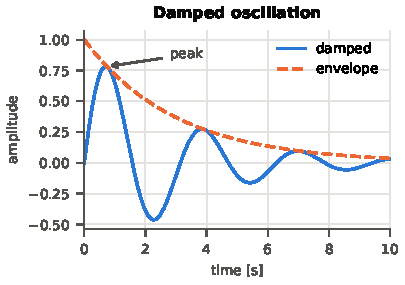
\includegraphics[width=\linewidth]{oo_example.pdf}

\vspace{2pt}
\raggedright
\begin{block}{Two interfaces}
|plt.plot(...)|: implicit ``current axes'', for quick looks.\\
|fig, ax = plt.subplots()|: explicit, \textbf{use it for real
code}.
\end{block}
\end{columns}
\end{frame}

% ---------------------------------------------------------------------
\begin{frame}[fragile]{Common plot types}
\begin{columns}[T]
\column{0.44\textwidth}
\begin{lstlisting}
fig, axs = plt.subplots(
    2, 2, layout="constrained")
axs[0, 0].plot(x, np.sin(x), label="sin")
axs[0, 0].plot(x, np.cos(x), label="cos")
axs[0, 0].legend()
axs[0, 1].scatter(xs, ys, s=6, alpha=0.7)
axs[1, 0].bar(["A", "B", "C", "D"],
              [42, 27, 31, 18])
axs[1, 1].hist(rng.normal(size=1000),
               bins=30)

titles = "Line Scatter Bar Histogram".split()
for ax, t in zip(axs.flat, titles):
    ax.set_title(t)
\end{lstlisting}
\hint{Also: \cc{barh}, \cc{errorbar}, \cc{fill\_between}, \cc{boxplot},
\cc{violinplot}, \cc{imshow}, \cc{contour}, \cc{stackplot}.}
\column{0.53\textwidth}
\centering
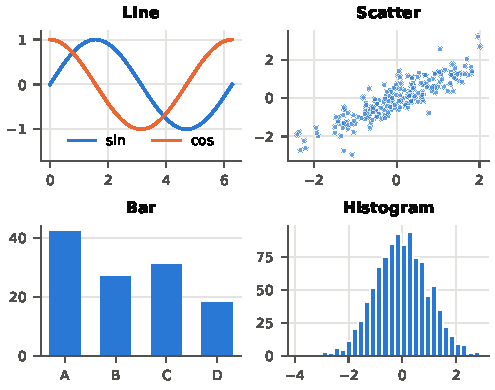
\includegraphics[width=\linewidth]{plot_types.pdf}
\end{columns}
\end{frame}

% ---------------------------------------------------------------------
\begin{frame}[fragile]{Customizing \& saving}
\begin{columns}[T]
\column{0.56\textwidth}
\begin{lstlisting}
plt.style.use("ggplot")         # plt.style.available
plt.rcParams["font.size"] = 11  # global defaults

fig, (ax1, ax2) = plt.subplots(1, 2, sharey=True,
                               figsize=(8, 3))
ax1.plot(x, y, color="tab:blue", linewidth=2,
         marker="o", linestyle="--")
ax1.grid(alpha=0.3)
ax1.set_xticks([0, 5, 10], ["start", "mid", "end"])
ax2.set_yscale("log")
fig.suptitle("Two panels, shared y-axis")

fig.savefig("plot.pdf")           # vector: pdf, svg
fig.savefig("plot.png", dpi=200)  # raster: png
\end{lstlisting}
\column{0.40\textwidth}
\begin{block}{pandas plots to Matplotlib}
\begin{lstlisting}[aboveskip=7pt]
ax = df.plot(x="month", y="sales",
             kind="bar")
ax.set_ylabel("sales")
\end{lstlisting}
|df.plot| returns an ordinary |Axes|, so everything on this slide
still applies.
\end{block}
\begin{itemize}\setlength\itemsep{3pt}
  \item |layout="constrained"| prevents overlapping labels.
  \item In Jupyter, figures render inline automatically.
  \item \textbf{seaborn} builds on Matplotlib for statistical plots.
\end{itemize}
\end{columns}
\end{frame}

% ---------------------------------------------------------------------
\begin{frame}[fragile]{Putting it together: NumPy $\rightarrow$ pandas $\rightarrow$ Matplotlib}
\begin{columns}[T]
\column{0.53\textwidth}
\begin{lstlisting}
rng = np.random.default_rng(42)
n, cities = 365, ["Tehran", "Berlin", "Tokyo"]
df = pd.DataFrame({
    "date":  pd.date_range("2025-01-01", periods=n),
    "city":  rng.choice(cities, size=n),
    "sales": rng.normal(100, 20, size=n).round(1),
})
monthly = (
    df.groupby([pd.Grouper(key="date", freq="ME"),
                "city"])["sales"]
      .sum()
      .unstack("city")        # cities -> columns
)
monthly.index = monthly.index.strftime("%b")
ax = monthly.plot(marker="o")
ax.set(ylabel="monthly sales")
\end{lstlisting}
\hint{\cc{freq="ME"} = month end. One expression turns 365 raw rows
into a 12\,$\times$\,3 table, ready to plot.}
\column{0.43\textwidth}
\centering
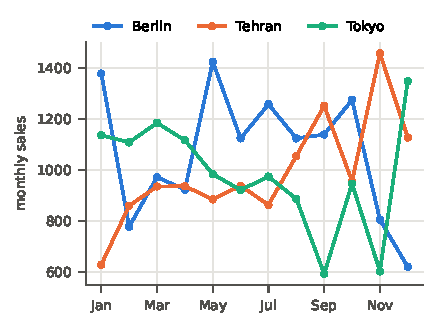
\includegraphics[width=\linewidth]{pandas_pipeline.pdf}

\hint{Synthetic data, generated by the code on the left.}
\end{columns}
\end{frame}

% =====================================================================
\begin{frame}{Where to go next}
\begin{columns}[T]
\column{0.50\textwidth}
\head{Official docs}
\begin{itemize}\setlength\itemsep{3pt}
  \item \emph{The Python Tutorial}: docs.python.org/3/tutorial
  \item \emph{NumPy: the absolute basics for beginners}, and
        \emph{NumPy for MATLAB users}: numpy.org/doc
  \item \emph{10 minutes to pandas}: pandas.pydata.org/docs
  \item \emph{Quick start guide}: matplotlib.org
\end{itemize}
\medskip
\head{Books}
\begin{itemize}\setlength\itemsep{3pt}
  \item \emph{Fluent Python}, Luciano Ramalho
  \item \emph{Python Data Science Handbook}, Jake VanderPlas
        (free online)
\end{itemize}
\column{0.44\textwidth}
\begin{exampleblock}{Take-aways}
\begin{enumerate}\setlength\itemsep{3pt}
  \item Names are references; know what is mutable.
  \item Iterate over things: comprehensions, \texttt{enumerate},
        \texttt{zip}.
  \item Use \texttt{with}, f-strings, \texttt{pathlib}, dataclasses.
  \item In NumPy and pandas, think in \emph{whole arrays and
        columns}, not loops.
  \item Plot with \texttt{fig, ax = plt.subplots()}.
\end{enumerate}
\end{exampleblock}
\end{columns}
\end{frame}

\begin{frame}[standout]
Questions?
\end{frame}

\end{document}
